\documentclass[11pt]{article}
\usepackage{geometry}                % See geometry.pdf to learn the layout options. There are lots.
\geometry{letterpaper} 
\usepackage[utf8]{inputenc} 
\usepackage{mathtools}                    % ... or a4paper or a5paper or ... 
%\geometry{landscape}                % Activate for for rotated page geometry
%\usepackage[parfill]{parskip}    % Activate to begin paragraphs with an empty line rather than an indent
\usepackage{graphicx}
\usepackage{amssymb}
\usepackage{epstopdf}
\usepackage{graphicx}
\usepackage[spanish]{babel}
\usepackage{float}

\title{Programación y Algoritmos I Tarea 9}
\author{Isabel López Huerta\\Ivonne Monter Aldana}
%\date{}                                           % Activate to display a given date or no date
\begin{document}

\maketitle

\begin{itemize}
 \item [\textbf{Problema 1}] [0.5 puntos]

Demostrar que si $r$ es la raíz de un árbol rojo-negro de altura $h$, tenemos 
\begin{align*}
h_b(r)\geq \frac{h}{2}
\end{align*}

\textbf{Respuesta:}

Como la altura es la longitud del camino más largo que comienza en la raíz y termina en una hoja, existe un camino $r-n_1-n_2-\cdots-n_h$ con $n_h$ una hoja, como $h_b(r)$ es el número de nodos negros de cualquier camino desde r a una hoja, en particular es igual al número de nodos negros del conjunto 
$\{n_1,\ldots,n_2\}$ más uno por el nodo NULL. Sea $p$ y $q$ el número de nodos rojos y negros respectivamente en el conjunto $\{n_1,\ldots,n_2\}$, entonces $h_b(r)=h-p+1$, por lo tanto $h_b(r)$ es inversamente proporcional a $p$, como no puede haber nodos rojos consecutivos, el número máximo de nodos rojos que puede haber se logra con $n_1$ rojo luego $n_2$ negro, $n_3$ rojo y así sucesivamente alternando entre rojo y negro. 

Si $h$ es par el número de rojos es $\frac{h}{2}$, entonces $h_b(r)=h-\frac{h}{2}+1=\frac{h}{2}+1$.

Si $h$ es impar, entonces $h=2k+1$ para algún $k$ y el número de rojos es igual a $k+1$, 
$h_b(r)=h-k-1+1=h-k=k+1=\frac{h}{2}+\frac{1}{2}$.

Por lo tanto
\begin{align*}
h_b(r)\geq \frac{h}{2}
\end{align*}
$\blacksquare$
\item [\textbf{Problema 2}] [0.5 puntos]

Demostrar por inducción sobre la altura de los nodos que un subarbol enraizado en un nodo v tiene
al menos $2^{h_b(v)} - 1$ nodos internos.

\textbf{Respuesta:}

Si la altura del sub arbol con raiz en v es 0 entonces $v=null$, y el subarbol enraizado en v tine $2^{h_b(v)} - 1=2^0-1=0$
Ahora si consideramos que v, con altura positiva y como padre de dos hijos tenemos que cada hijo tiene que tener una altura negra de  $h_b(v)$ si es un nodo rojo y de $h_b(v)-1$ si es un nodo negro, por lo que por hipotesis de inducción almenos cada hijo de v tendra $2^{h_b(v)-1} - 1$ nodos internos, por lo que los nodos internos del subarbol enraisado en v seran almenos $(2^{h_b(v)-1} - 1)+(2^{h_b(v)-1} - 1)+1=2^{h_b}-1$ $\blacksquare$

 \item [\textbf{Problema 3}] [0.5 puntos]

Deducir de lo anterior que, si n es el número total de nodos, la altura h del arbol satisface:
\begin{align*}
h\leq2\log_2(n+1)
\end{align*}

\textbf{Respuesta:}

Como consecuencia de las dos preguntas anteriores podemos afirmar que
\begin{align*}
   n&\geq2^{h_b(r)}-1
  \\ \xrightarrow{}  n+1&\geq2^{h_b(r)}
\end{align*}
 por la pregunta uno se cumple la desigualdad
\begin{align*}
    2^{\frac{h}{2}}&<2^{h_b} 
   \\ \xrightarrow{} n+1&\geq 2^{\frac{h}{2}}
\end{align*}
aplicamos logaritmo
\begin{align*}
\log(n+1)\geq \frac{h}{2}
\end{align*}
multiplicamos por 2
\begin{align*}
h\leq 2 \log(n+1).
\end{align*}

\item [\textbf{Problema 4}] [0.5 puntos]

Definimos la inserción de un nuevo dato en un árbol rojo-negro como sigue: Insertamos el nuevo nodo
$w$ como en un ABB normal (bajando hacia su lugar, por búsqueda) y lo coloreamos como rojo. Si
ese nodo es la raíz ($w$ fue el primer nodo), lo coloreamos como negro. Mostrar que el único caso en
que se puede generar una violación de las reglas de árbol rojo-negro es cuando el padre de $w$ es rojo.

\textbf{Respuesta:}

Al insertar el nuevo nodo $w$ en color rojo, ninguna altura negra se ve afectada, ya que son el número de nodos negros,por lo que propiedad 5 se conserva. Ahora como el nuevo nodo es una hoja no tiene hijos y si el nodo padre es negro, entonces la propiedad de no tener nodos rojos consecutivos se conserva. Si el nodo padre es rojo entonces tenemos dos nodos rojos consecutivos que es una violación a la propiedad tres.

\item [\textbf{Problema 5}] [0.5 puntos]

 Mostrar que, en el caso anterior de violación, si el nodo tío de w (es decir, el otro hijo de su abuelo)
es también rojo, hay una correción muy simple que se puede hacer al cambiar de colores el abuelo, el
papa y el tío. Cómo cambia la altura negra de los nodos del árbol con esta correción? Mostrar que la
correción puede provocar una violación al nivel el abuelo. Cuál es la complejidad total de la correción?

\textbf{Respuesta:}

En la figura 1 el abuelo del nuevo nodo a insertar es la raíz, como su papa es rojo se incumple las propiedades del árbol RN por lo que se cambia a papa y tío a negro y el abuelo pasa a ser rojo, pero como la raíz del árbol siempre tiene que ser negra se cambia a negra.
\begin{figure}[H]
    \centering
    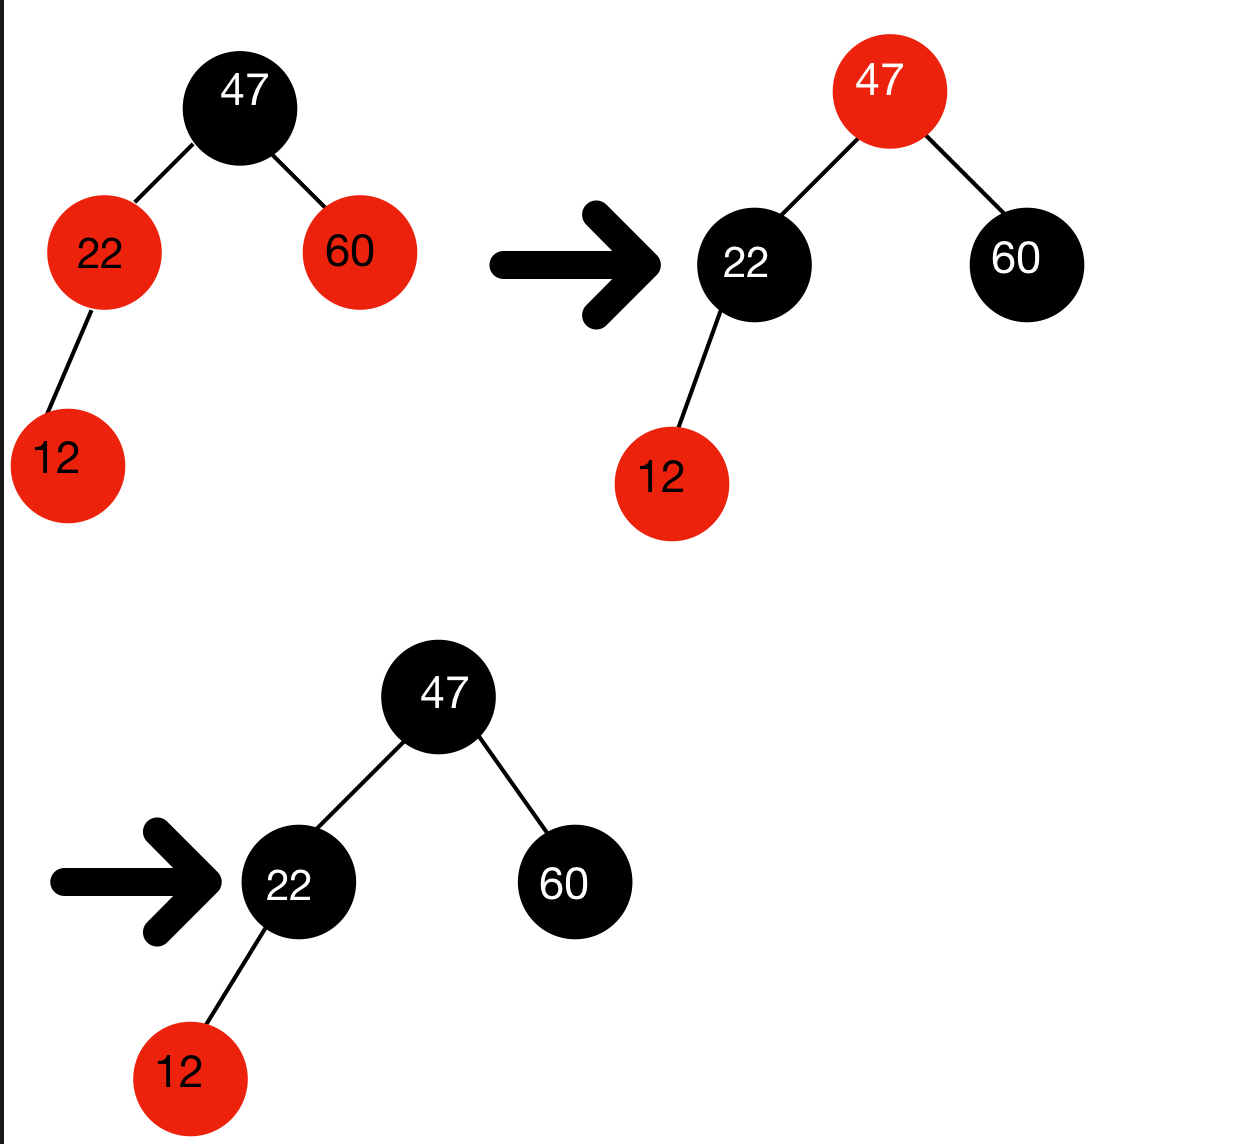
\includegraphics[scale=.15]{IMG-2099.jpg}
    \caption{El abuelo del nuevo nodo es la raiz.}
    \label{}
 \end{figure}
En la figura 2 papa y tío son rojos y su abuelo negro, al entrar  un nuevo nodo rojo se incumple las propiedades del árbol RN, por lo que  cambia de color el papá, pasa a ser negro, y el abuelo pasa a ser rojo, con lo que el tío tiene que pasar a ser negro para cumplir todas las propiedades del árbol RN.   

Hay que considerar que se puede dar el caso donde el papa del abuelo puede ser rojo despues del cambio al padre del nuevo nodo, lo que nos dejaria con dos nodos rojos consecutivos, esto incumple las propiedades el arbol RN, este caso se aborda en la siguiente pregunta.
\begin{figure}[H]
    \centering
    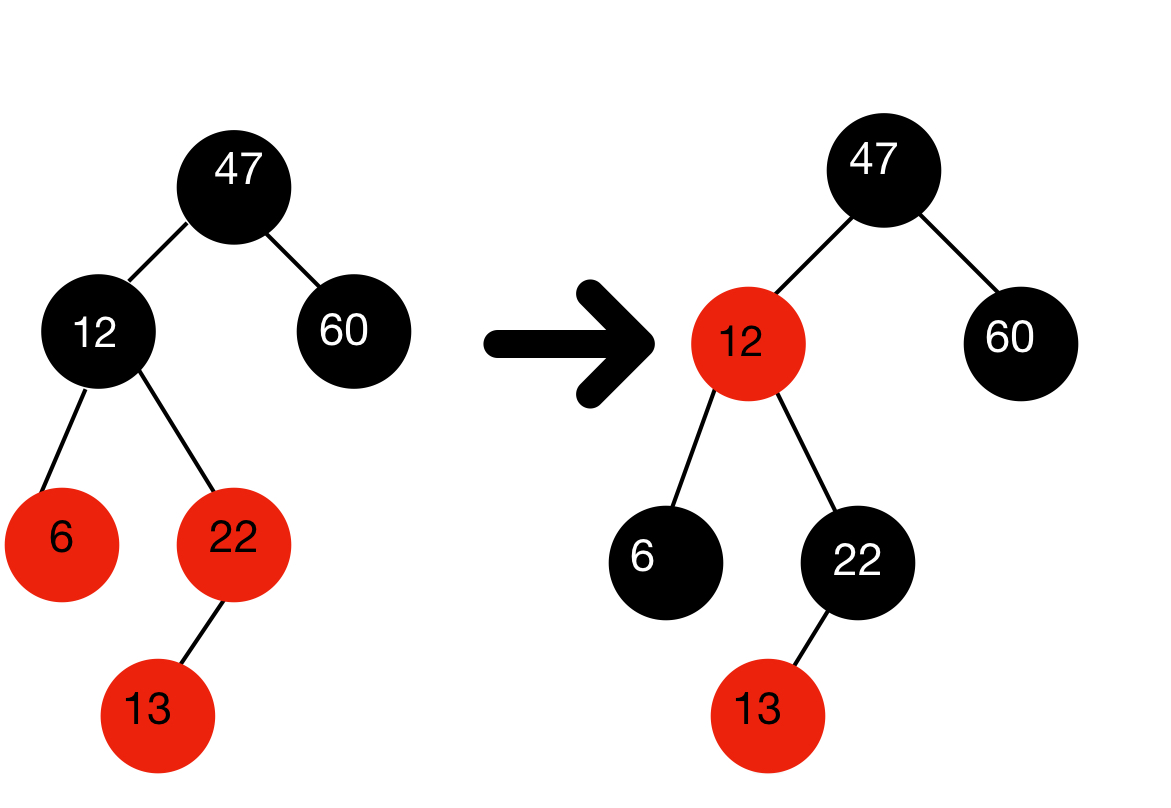
\includegraphics[scale=.2]{IMG-2100.jpg}
    \caption{El abuelo del nuevo nodo es la raiz de un subarbol.}
    \label{}
 \end{figure}
 Cada que se presenta este caso, la altura negra del abuelo aumenta un grado, ya que cuando calculamos la altura negra no se cuenta el nodo al que se le quiere calcular, y ahora se agrego un nodo negro ya que el papa paso de rojo a negro y el tío también, esto permite que se mantengan  equilibradas las alturas, sin embargo, los nodos ascendentes del abuelo no sufren cambios por que ya consideraban ese nodo negro con el abuelo.
 
\item [\textbf{Problema 6}] [0.5 puntos]

Mostrar que en el otro caso (si el tío es negro), se puede usar las mismas rotaciones que vimos en el caso de árboles AVL para corregir el árbol rojo-negro. ¿Cómo cambia la altura negra de los nodos del árbol con esta correción? ¿Cuál es la complejidad de esta correción?

\textbf{Respuesta:}
Para hacer al análisis se dividió el problema en los siguientes casos:
\begin{itemize}
\item Caso 1

Se inserta el nodo $w$ con el color rojo del lado derecho de $x$.
$x$ es un nodo rojo y es hijo izquierdo. El tío de $w$, la raíz del subárbol $T2$ es negro.
Como $x$ es rojo, su padre $y$ debe ser negro, ya que antes de insertar $w$, el árbol cumplía todas las condiciones.

Se hace una rotación derecha de $y$.

Entre $y$ y $w$ originalmente había un solo nodo negro ($y$), al hacer la rotación entre $x$ y $w$ hay un solo nodo negro ($x$) por lo que los caminos que pasaban por $y ->w$ que ahora pasan por $x->y$ siguen teniendo la misma altura.

Análogamente para los caminos que pasaban por $y->T2$, había dos nodos negros, al hacer una rotación se remplaza por $x->T2$, donde también hay dos nodos negros,por lo tanto la altura se conserva. Lo mismo para el camino $x->T1$, en el que se agregó el nodo rojo $y$, por lo que no hay cambios en la altura negra.
\begin{figure}[H]
\begin{center}
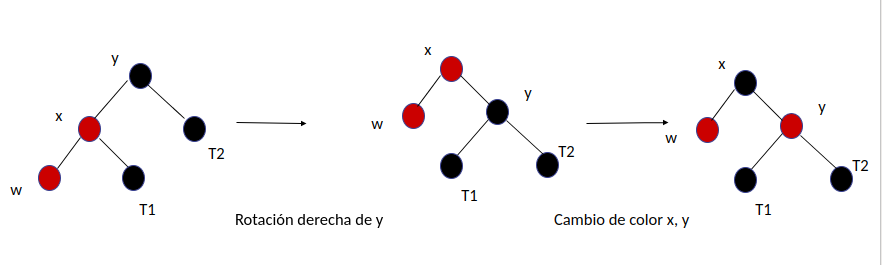
\includegraphics[scale=0.5]{caso1.png}
\caption{Caso 1}
\end{center}
\end{figure}

\item Caso 2

Se inserta el nodo $w$ con el color rojo del lado derecho de $x$. $x$ es un nodo rojo y es hijo derecho. El tío de $w$, la raíz del subárbol $t2$ es negro

Como $x$ es rojo, su padre $y$ debe ser negro, ya que antes de insertar $w$, el árbol cimplia las condiciones.

Se cambian de color $x$ y $y$.

Se hace una rotación derecha de $y$, los nuevos caminos preservan el número de nodos negros que los anteriores.

El camino de $y->T2$ se remplazó por $x->T2$ en ambos hay dos nodos negros; el camino de $y->w$ se remplazó por $x->w$ en ambos hay un nodo negro; el camino de $y->T1$ se remplazó por $x->T1$, ambos tienen dos nodos negros. Por lo tanto las alturas negras de conservan
\begin{figure}[H]
\begin{center}
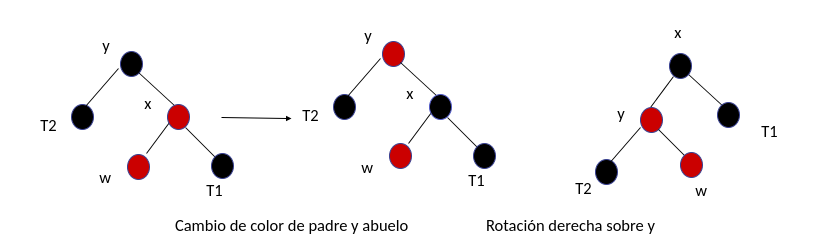
\includegraphics[scale=0.5]{caso2.png}
\caption{Caso 2}
\end{center}
\end{figure}

\item Caso 3

Se inserta el nodo $w$ con el color rojo del lado izquiero de $x$, $x$ es un nodo rojo y es hijo izquiero. El tío de $w$, la raíz del subábol $T2$ es negro.

Como $x$ es rojo, su padre $y$ deber ser negro, ya que antes de insertar $w$, el árbol cumplia todas las condiciones.

Se hace una rotación izquierda de $x$, lo que reduce el caso al anterior.
\begin{figure}[H]
\begin{center}
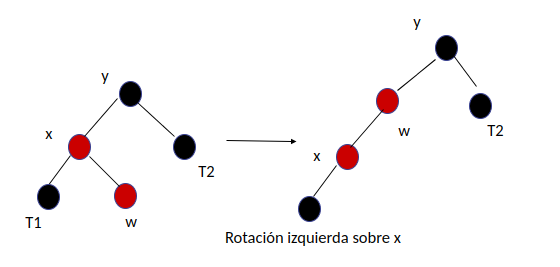
\includegraphics[scale=0.5]{caso3.png}
\caption{Caso 3}
\end{center}
\end{figure}

\item Caso 4

Se inserta el nodo $w$ con el color rojo del lado derecho de $x$. $x$ es un nodo rojo y es hijo derecho. EL tío de $w$, la raíz del subárbol $T2$ es negro.

Como $x$ es rojo, su padre $y$ debe ser negro, ya que antes de insertar $w$, el árbol cumplía con todas las condiciones.

Se hace una rotación izquierda de $y$ y cambio de color de $x$ y $y$.

El camino $y->T2$ se remplazó por $x->T2$, ambos tienen dos nodos negros; el camino $y->w$ se remplazó por $x->w$ ambos tienen dos nodos negros; el camino $y->T1$ se remplazó por $x->T1$ ambos tiene dos nodos negros. 
Por lo tanto las alturas se conservan 
\begin{figure}[H]
\begin{center}
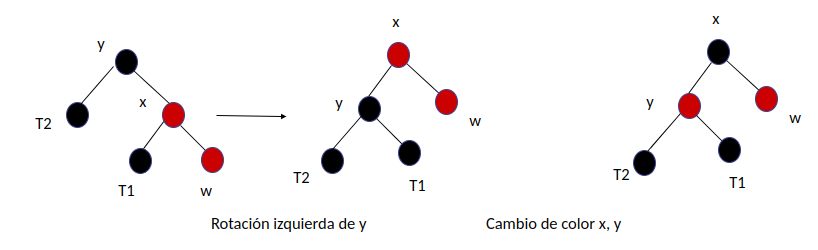
\includegraphics[scale=0.5]{caso4.png}
\caption{Caso 4}
\end{center}
\end{figure}

\item Caso 5
Se inserta el nodo $w$ con el color rojo del lado izquierdo de $x$. $x$ es un nodo rojo. El tío de $w$, la raíz del subárbol $T2$ es rojo.

Como $x$ es rojo, su padre $y$ debe ser negro, ya que antes de insertar $w$, el árbol cumplía todas las condiciones.

Al intercambiar los colores las alturas negras se conservan. Se traslada la dificultad al nodo $y$, ya que si su padre es rojo hay una violación a las propiedades del árbol y caería en alguno de los casos ya mencionados, incluido este.
\begin{figure}[H]
\begin{center}
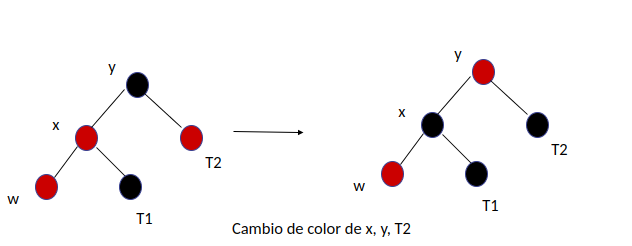
\includegraphics[scale=0.5]{caso5.png}
\caption{Caso 5}
\end{center}
\end{figure}
\end{itemize}
Los casos $1,2,3,4$ se arreglan en tiempo constante, haciendo una rotación y/o cambio de colores, en el peor de los casos cada vez se cae en el caso 5, lo que hace que el error se propagué hasta la raíz, si se comienza desde el último nivel, se tendrían que realizar tantos cambios como niveles y por el ejercicio tres la correción tendría una complejidad $O(\log(n))$.

\end{itemize}


\end{document}  
